\subsection{\textbf{Future Research}}
\begin{wrapfigure}{r}{110pt}
    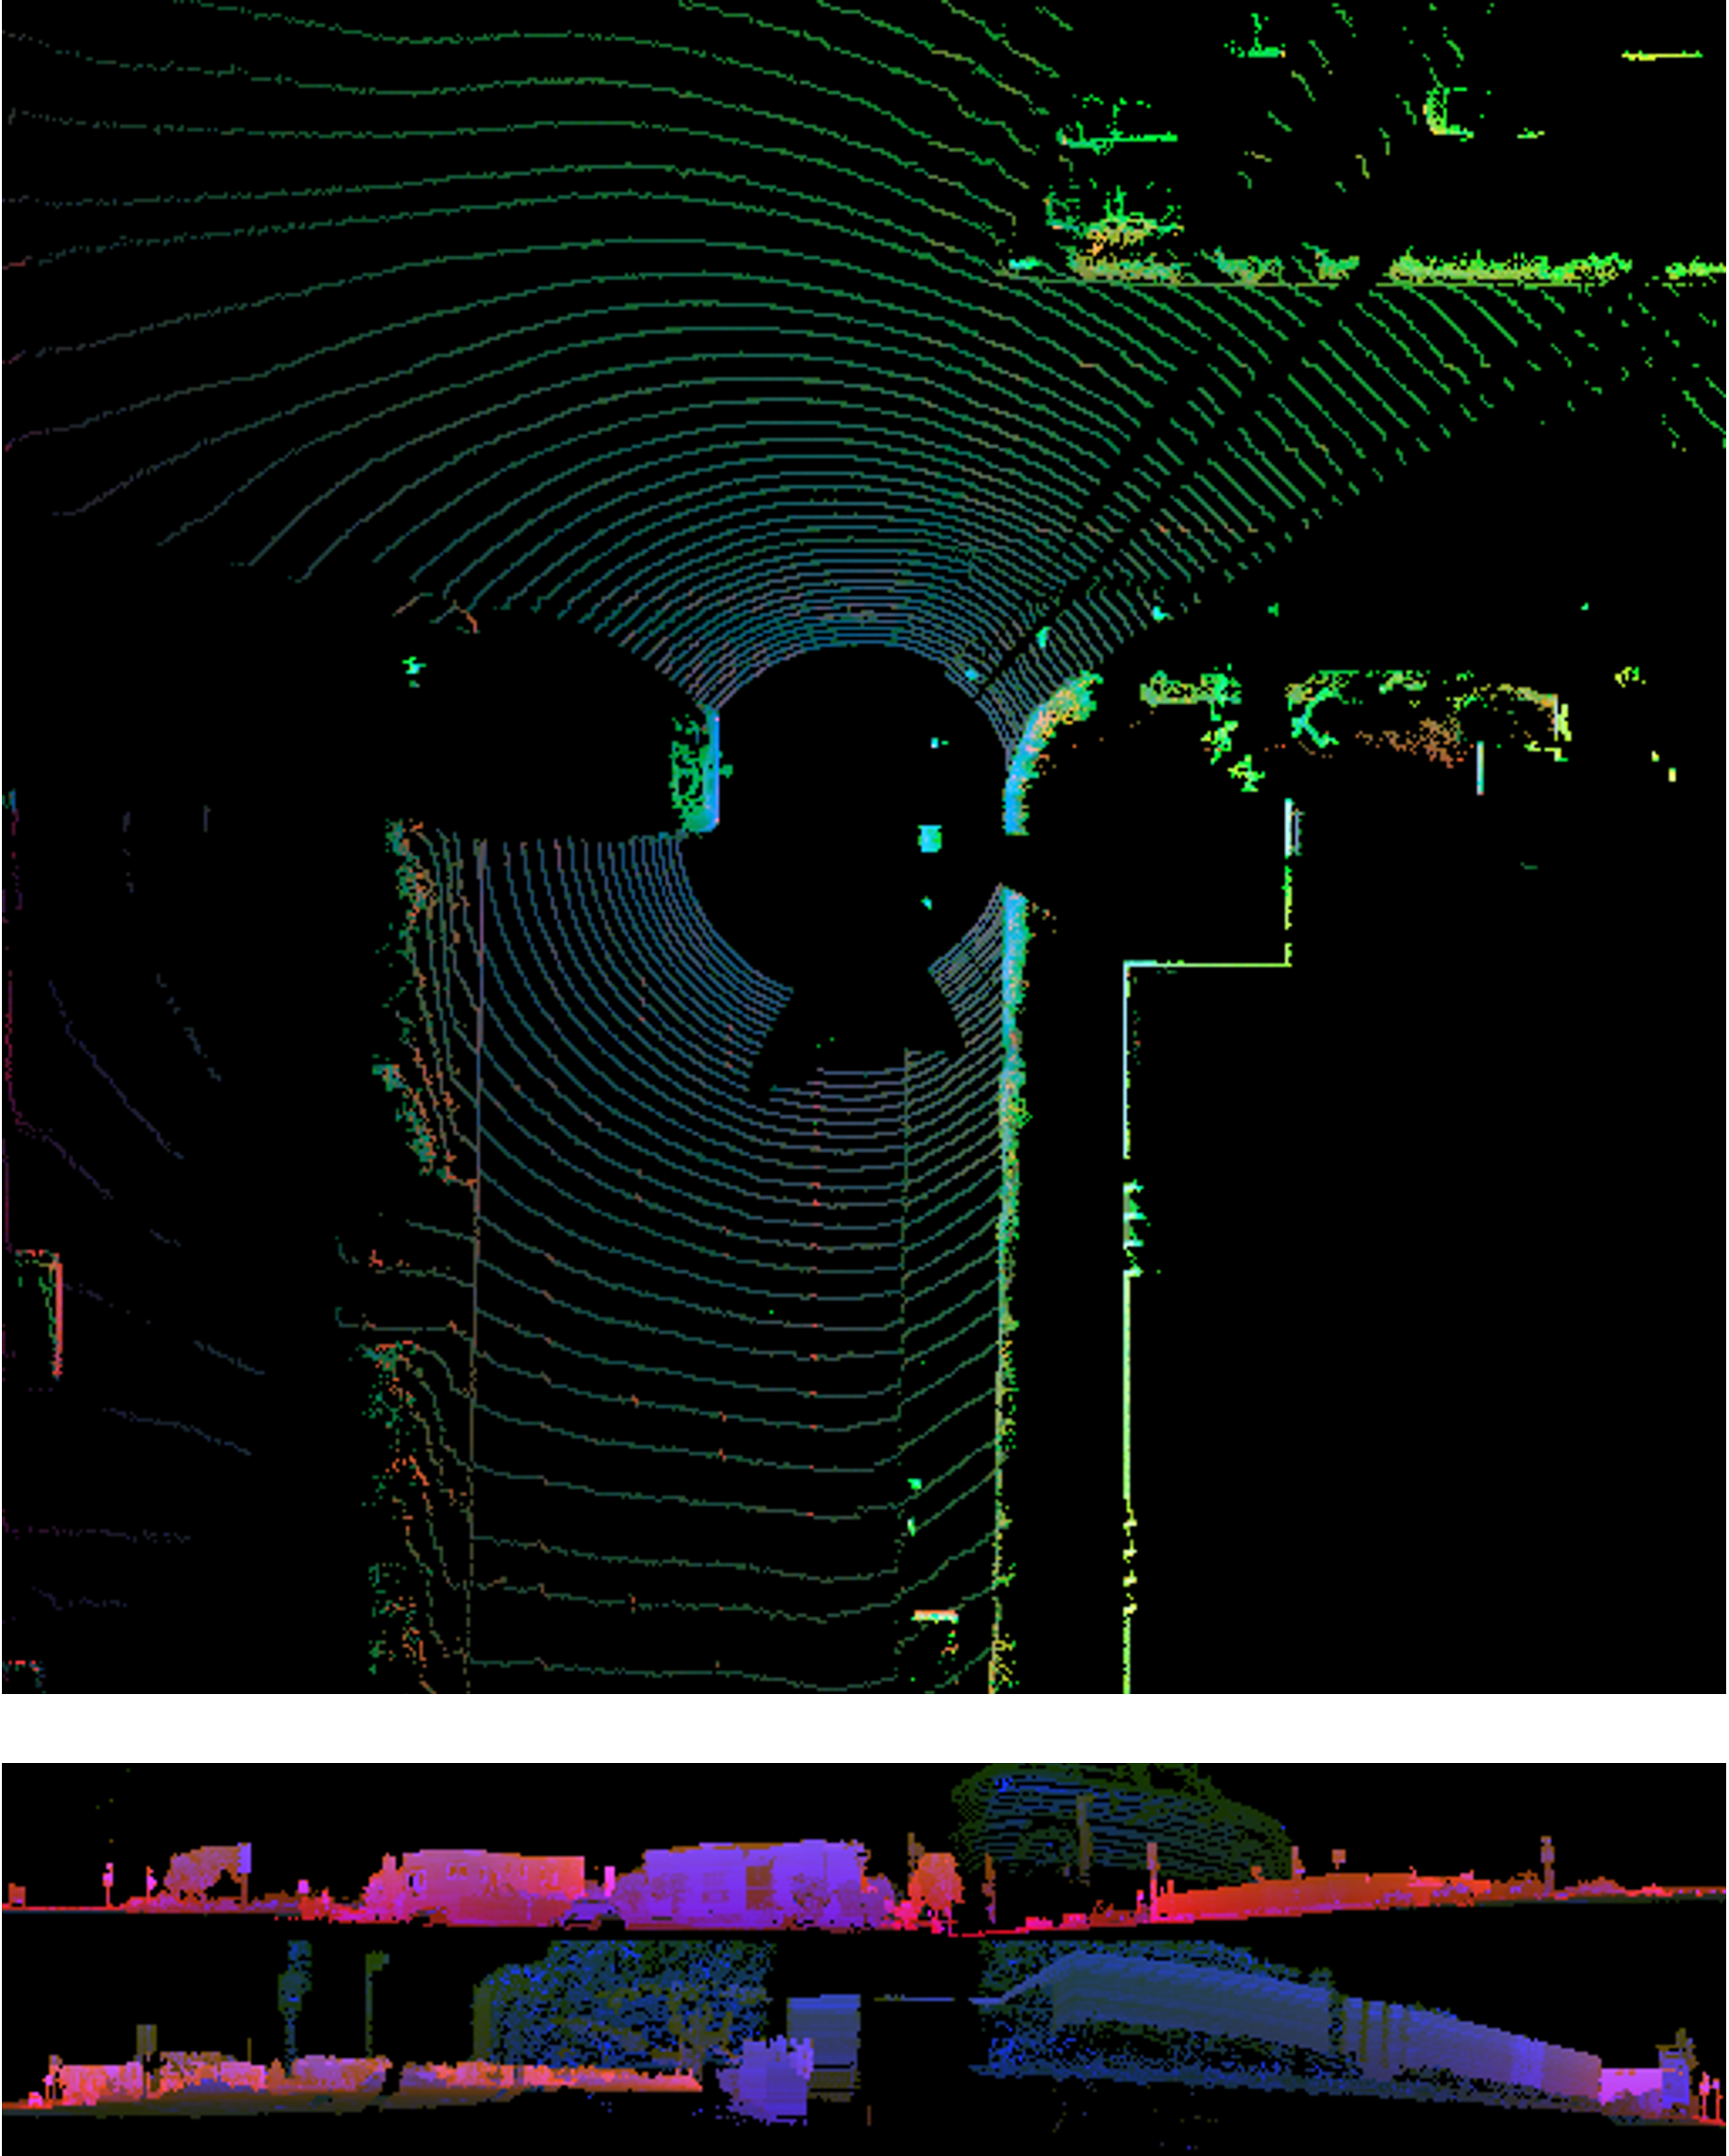
\includegraphics[width=110pt]{pic/fusion.png}
    \mainfont\fontsize{9pt}{9pt}\selectfont\caption{ \mainfont\fontsize{9pt}{9pt}\selectfont Multi view fusion with bird's eye view and spherical view}
    \label{fig:fusion}
    \end{wrapfigure}
My future research will continue to focus on computer vision, with a particular emphasis on scene understanding and perception. Additionally, I intend to expand my research scope to encompass new fields beyond object detection. In addition to investigating the potential of masked modelling, I am interested in examining other self-supervised and semi-supervised learning techniques. 

The development of pixelNeRF \cite{pixelnerf} opened the line of research of utilising NeRFs for conditioned scene rendering. The development of 3D Gaussian splatting, and more recently methods such as MVSplat \cite{mvsplat} 3D Gaussian representations are obtained with single forward pass, while also rendering them in real-time. The 3D Gaussians are a unique latent space for 3D scene representations, offering many new research avenues to explore. To illustrate the authors of S4C \cite{s4c} employ a pixelNeRF to perform 3D semantic scene completion without the need for 3D annotations in a self-supervised manner. I am interested in developing similar methods that make use of the fast rendering of 3D Gaussians for scene understanding.

Methodically I am particular interested in developing and focusing on training strategies such as regularizing via multi task and curriculum learning. For example the authors of ProFusion3D \cite{valada} present an impressive multimodal fusion pipeline, while also focusing on novel training strategies via additional objectives, such as denoising, in the pretraining phase. 